\documentclass[main.tex]{subfiles}

\begin{document}

\chapter{Gewöhnliche Differentialgleichungen}


\section{Einleitung}

\begin{Definition}
  Wir suchen eine (unbekannte) Funktion $u$, die reell- oder verktorwertig ist und folgenden 2 Bedingungen genügt:
  \begin{enumerate}
    \item Sie erfüllt Differentialgleichung(en), das heißt Gleichungen zwischen $u$, Ableitungen von $u$ und vorgegebenen Funktionen.
    \item Sie erfüllt Nebenbedingungen (genannt Anfangs- oder Randbedingungen), das heißt spezielle Werte von $u$ und ihren Ableitungen.
  \end{enumerate}

  Als \textbf{gewöhnlich} bezeichnen wir Differentialgleichungen, die wir mit $u$ als Funktion in einer Variablen lösen können.

  Dem gegenüber sind \textbf{partielle} Differentialgleichungen solche, die durch Funktionen in mehreren Variablen gelöst werden.
\end{Definition}

\begin{Beispiel}[Allgemein]
  Betrachten wir
  \begin{equation*}
  t \cdot u''(t) = \cos(t) \cdot U(t)^2 \tag{*}
  \end{equation*}
  $$u(0) = 0 \qquad u'(0) = 1$$
  dann müssen wir erst entscheiden, in welchem Lösungsraum wir uns mit diesem Problem beschäftigen wollen. Wir könnten beispielsweise nach Lösungen in $\mathcal{C}^2 ((-\pi,\pi))$ suchen.

  Genauer haben wir dann in $(*)$ eine \textbf{nichtlineare}, gewöhnliche Differentialgleichung.
\end{Beispiel}

\begin{Beispiel}[Die biharmonische Gleichung]
  Wir betrachten eine elastische Platte, auf die wir mit einer Kraft einwirken (also existiert ein Kraftfeld).
  \incfig{biharmonisch}
  Für $u(x,y)$, der Höhe der Platte bei $(x,y) \in B$, gilt:
  \begin{equation*}
    u_{xxxx} + 2 \cdot u_{xxyy} + u{yyyy} := \dfrac{\partial^4}{\partial x^4} u + \dfrac{\partial^4}{\partial x^2 \partial y^2} u + \dfrac{\partial^4}{\partial y^4}= -f(x,y) \tag{*}
  \end{equation*}
  Zudem haben wir Randbedingungen: $U(x,y) = 0 \A (x,y) \in \partial B$

  Alternative Schreibweise: $\delta^2 u = -f$ oder $\nabla^4 u = -f$.

  Wir können zu $(*)$ sagen, dass die Gleichung \textbf{linear} in $u$ ist. Somit haben wir eine \textbf{lineare} partielle Differentialgleichung vom Grad 4.

  Zudem ist sie \textbf{homogen} im Spezialfall $f = 0$ und sonst inhomogen.
\end{Beispiel}

\begin{Beispiel}[Ricatti-Gleichung]
  Für $u$, eine Funktion in einer Variablen:
  $$u'(x) = a_0(x) + a_1(x) \cdot u(x) + a_2(x) \cdot u(x)^2$$
  Als Differentialgleichung ist die Gleichung gewöhnlich, aber nicht linear, erster Ordnung.
  Sie ist wichtig in der Kontroll-/Transporttheorie.
\end{Beispiel}
Eng verwandt ist

\begin{Beispiel}[Bernoull-Gleichung]
  Ein Gleichung der Form
  $$y' + Py = Qy^n$$
  Achtung: hier ist $y$ eine Funktion: $y = y(x)$
\end{Beispiel}

\begin{Beispiel}[Minimalflächengleichung (Lagrange, 1762)]
  Wir betrachten $c$, eine $1$-dimensionale Mannigfaltigkeit im $\R^3$ (also konkret geschlossene Kurven). Nun suchen wir die Fläche $F$ mit $\partial F = c$, deren Fläche minimal ist.

  Lokal können wir diese Minimalfläche als Graph einer Funktion $u = u(x,y)$ schreiben, die erfüllt
  $$(1 + u_x^2) u_{yy} - 2u_x u_y u_{xy} + (1+u_y^2)u_{xx} = 0$$
  Hier ist also eine partielle, nichtlineare Differentialgleichung.
\end{Beispiel}

\begin{Beispiel}
  Sei $U \subseteq \R^n$ offen und $F: U \to \R^n$ ein Vekorfeld. Betrachten wir $u(t)$ als die Position eines Partikels, das von $F$ beeinflusst wird. Wir setzen $u(0) = x_0 \in U$ (Anfangsbedingung).

  Wir haben
  \begin{equation*}
    u'(t) = F(u(t)) \tag{*}
  \end{equation*}

  Diese Differentialgleichung ist \textbf{autonom}, da $F$ nicht von $t$ abhängt.

  Für $n = 2$ und $F(x,y) = (y,-x)$ dann vereinfacht sich $(*)$ zum folgenden System
  $$\left\{\begin{aligned}
    u_1' & = u_2 \\ u_2' & = -u_1
  \end{aligned}\right. \Leftrightarrow u'(t) = \begin{pmatrix}
    0 & -1 \\ 1 & 0
  \end{pmatrix} \cdot u(t)$$

  Ist $F$ zeitabhängig, also $F: I \times U \to \R^3$ mit $I$, einem Intervall, so bekommen wir:
  $$u'(t) = F(t,u(t))$$
  Diese Differentialgleichung ist nicht autonom.
\end{Beispiel}


\section{Differentialgleichungssysteme}

Wir betrachten $U \subseteq \R^n$ offen und haben dazu dann den Ring $\mathcal{C}^\infty(U)$.

\begin{Definition}[Lineare Differentialoperatoren]
  Eine lineare Abbildung
  $$\begin{aligned}
    L : \mathcal{C}^\infty(U) & \to \mathcal{C}^\infty(U) \\
    u & \mapsto \sum \limits_\alpha a_\alpha \cdot \partial_1^{\alpha_1} \partial_2^{\alpha_2} ... \partial_n^{\alpha_n} \cdot u
  \end{aligned}$$
  nennt man \textbf{linearen Differentialoperator}.

  (wir haben $\alpha = (\alpha_1,...,\alpha_n) \in K_{\geq 0}^n$ und $a_\alpha \in \mathcal{C}^\infty(U)$ mit Koeffizienten $(a_\alpha)_\alpha$)

  Eine homogene Gleichung ist dann der Form $L \cdot u = 0$, und in inhomogen erhält man $L \cdot u = b$.
  \begin{Bemerkung}
    Wenn wir algebraisch $\mathcal{C}^\infty(U)$ als Vektorraum auffassen, dann wird $L$ zu einem Vektorraumisomorphismus und es gilt:
    $$L \cdot u = 0 \Leftrightarrow u \in \ker(L)$$
    $$L \cdot u = f \Leftrightarrow f \in \text{im}(L)$$
    Lieber suchen wir aber nach dem Quotientenraum $\mathcal{C}^\infty(U) / \text{im}(L) := \text{coker}(L)$.
  \end{Bemerkung}

  Man nennt $f$ \textbf{Störfunktion}.
\end{Definition}

\begin{Beispiel}[Laplace-operator]
  $$\Delta u = \sum \limits_{i = 1}^n \partial_i \partial_i u$$
  Also für $u = u(x,y)$:
  $$\Delta u = \dfrac{\partial^2}{\partial x^2}u + \dfrac{\partial^2}{\partial y^2} u$$
  Wir können auch schreiben
  $$\Delta u = tr(D^2 u)$$
  Dieser Operator tritt beispielsweise in Wärmetransferproblemen auf.
\end{Beispiel}

Genauer betrachten wir:

\subsection{Algebraische Überlegungen zu Differentialgleichungen}

\begin{Definition}[Differentialring]
  Ein \textbf{Differentialring} (oder eine Differentialalgebra) ist ein kommutativer Ring $R$ zusammen mit einer Abbildung $\partial: R \to R$, die erfüllt
  \begin{itemize}
    \item $\partial(a+b) = \partial(a) + \partial(b)$
    \item $\partial(a \cdot b) = \partial(a) \cdot b + a \cdot \partial(b)$
  \end{itemize}
\end{Definition}

\begin{Beispiel}
  \begin{itemize}
    \item $R = \mathcal{C}^\infty(I)$ mit $I \subseteq \R$, einem Intervall und $\partial a := a'$
    \item $R = \C[t]$ mit $\partial P = P'$ (also $\partial1 = 0$ und $\partial t = 1$)
    \item $R = \C[\![t]\!]$ (Potenzreihen) mit $\partial \sum \limits_{n=0}^\infty a_n t^n = \sum \limits_{n=0}^\infty n \cdot a_nt^{n-1}$
  \end{itemize}
  Statt $\C$ können wir auch andere Körper verwenden, insbesondere auch eindliche Körper $F_p$.
\end{Beispiel}

Wir können ein System also als vektorwertige Funktion auffassen mit einem Matrix-artigen Linearoperator und uns nun Problemen wachsender Komplexität zuwenden:


\section{Lineare gewöhnliche Differentialgleichungen}

Wir betrachten
\begin{equation*}
  L \cdot u = 0 \quad L \cdot u = a_d u^{(d)} + ... + a_2 u'' + a_1 u' + a_0 u \tag{*}
\end{equation*}
mit $a_d \in \mathcal{C}^\infty(I)$.
\\\\
\begin{minipage}{0.5\textwidth}
  Schreibe dann
  \begin{itemize}
    \item $u_0 = u$
    \item $u_1 = u'$
    \item $u_2 = u ''$
    \item $\vdots$
    \item $u_{d-1} = u^{(d-1)}$
  \end{itemize}
\end{minipage}
\begin{minipage}{0.5\textwidth}
  Dann können wir folgende Relationen aufstellen
  \begin{itemize}
    \item $u_1 = u_0'$
    \item $u_2 = u_1'$
    \item $\vdots$
    \item $u_{d-1} = u_{d-2}'$
  \end{itemize}
\end{minipage}
\\\\
Wir fassen lesbarer zusammen, als Matrix. Falls $a_d = 1$:
$$\begin{pmatrix}
  u_0 \\ u_1 \\ \vdots \\ \vdots \\ u_{d-1}
\end{pmatrix}' = \begin{pmatrix}
  0 & 1 & 0 & 0 & \dots & 0 \\
  0 & 0 & 1 & 0 & \dots & 0 \\
  \vdots & & & \ddots & & \vdots \\
  0 & 0 & \dots & 0 & 1 & 0 \\
  -a_0 & -a_1 & -a_2 & \dots & \dots & -a_{d-1}
\end{pmatrix} \cdot \begin{pmatrix}
  u_0 \\ u_1 \\ \vdots \\ \vdots \\ u_{d-1}
\end{pmatrix}$$
Also erhalten wir zu $(*)$ \textbf{äquivalent}
$$u' = A \cdot u$$
Wieso? Es existiert eine bijektion zwischen beiden Lösungsräumen. (Diese ist sogar kanonisch?)

\subsection{Konstante Koeffizienten}

Sei unser Differentialoperator
$$L:= \partial^d + a_{d-1} \partial^{d-1} + ... + a_2 \partial^2 + a_1 \partial + a_0$$
Also haben wir für eine Funktion $u$:
$$Lu = u^{(d)} + a_{d-1} u^{(d-1)} + ... + a_2 u'' + a_1 u' + a_0 u$$
mit $a_0, ..., a_{d-1} \in \C$, $L \in \C[\partial]$.

Äquivalent zu $Lu = 0$ ist das Differentialgleichungssystem $u' = Au$ für $A$ die \textbf{Begleitmatrix} von $L$ (also $\in M(d \times d, \C)$).

Wir erkennen, dass dies von einer Exponentialfunktion erfüllt wird, also setzen wir:
$$u(t) = \exp(A \cdot t) = \sum \limits_{n=0}^\infty \dfrac{A^n}{n!}t$$
und es gilt weiterhin $u'(t) = A \cdot u(t) (++)$.

Also ist Jede Spalte von $U(t)$ eine Lösung von $(*)$. Auch jede Linearkombination (mit Koeffizienten in $\C$) erfüllt dies. Konkret entspräche das der Multiplikation der Matrix mit einem Vektor:
$$\A x = \begin{pmatrix}
  x_0 \\ \vdots \\ x_{d-1}
\end{pmatrix}\in \C^d : u*(t) := u(t) \cdot x \textbf{ erfüllt } u*'(t) = A u*(t)$$

Wir fassen zusammen:
\begin{Theorem}
  Das Differentialgleichungs-Problem
  $$u' = A \cdot u \qquad u(0) = x$$
  mit $A \in M(d \times d, \C)$ und $r \in \C^d$ hat eine Lösung in jedem der Ringe
  $$\C^\infty(\R), \C^\infty(-1,1),...,\C[\![t]\!], ...$$
  Diese Lösung ist dann gegeben durch:
  $$u(t) = \exp(A \cdot t) \cdot x$$
  In diesen Differentialringen ist dies sogar die \textbf{einzige Lösung}.
\end{Theorem}

\begin{Beweis}
  Sei $v(t)$ eine Lösung von $v' = A \cdot v$ mit $v(0) = x$. Wir setzen
  $$w(t) := \exp(-A \cdot t) \cdot v(t)$$
  $$w(t)' = -A \cdot \exp(-A \cdot t) \cdot v(t) + \exp(-A \cdot t) \cdot A \cdot v(t) {\color{olive} = 0}$$
  Außerdem indentifizieren wir $w \equiv x$, also $w(0) = x$.

  Dann finden wir
  $$\begin{aligned}
    v(t) & = \exp(A \cdot t) \underbrace{\exp(-A \cdot t) \cdot v(t)}_{x} \\
    & = u(t)
  \end{aligned}$$
  Also war unsere anfängliche Lösung eindeutig.
\end{Beweis}

\begin{Beispiel}
  Wir betrachten
  $$L \cdot u = 0 \text{ mit } L \cdot u = u'' + u \Leftrightarrow u'' = -u$$
  Äquivalent ist die Formulierung (in 2D)
  $$u = \begin{pmatrix}
    u_1 \\ u_2
  \end{pmatrix} \qquad u' = A \cdot u \qquad A = \begin{pmatrix}
    0 & 1 \\ -1 & 0
  \end{pmatrix}$$
  Also haben wir $u(t) = \exp(A \cdot t)$.

  Nun ist $A$ diagonalisierbar mit
  $$A = S D S^{-1} = \begin{pmatrix}
    1 & 1 \\ -i & i
  \end{pmatrix} \cdot \begin{pmatrix}
    i & 0 \\ 0 & -i
  \end{pmatrix} \cdot \dfrac{1}{2}\begin{pmatrix}
    1 & i \\ 1 & -i
  \end{pmatrix}$$
  Also können wir umschreiben
  $$\begin{aligned}
    u(t) = S \cdot \exp(D \cdot t) \cdot S^{-1} & = S \cdot \begin{pmatrix}
      \exp(i \cdot t) & 0 \\ \exp(i \cdot t) & 0
    \end{pmatrix} \cdot S^{-1} \\
    & = \begin{pmatrix}
      -\sin(t) & \cos(t) \\ - \cos(t) & -\sin(t)
    \end{pmatrix}
  \end{aligned}$$
\end{Beispiel}

\begin{Beispiel}
  Wir nehmen jetzt
  $$L \cdot u = u''' - 3 u'' + 3u' -u$$
  Äquivalent können wir formulieren:
  $$u' = A \cdot u = \begin{pmatrix}
    0 & 1 & 0 \\ 0 & 0 & 1 \\ 1 & -3 & 3
  \end{pmatrix} \cdot u$$
  Hier berechnen wir die Jordan-Normalform:
  $$A = SJS^{-1} \Leftrightarrow
  \begin{pmatrix}
    0 & 1 & 0 \\ 0 & 0 & 1 \\ 1 & -3 & 3
  \end{pmatrix} = \begin{pmatrix}
    1 & -2 & 3 \\ 1 & -1 & 1 \\ 1 & 0 & 0
  \end{pmatrix} \cdot \begin{pmatrix}
    1 & 1 & 0 \\ 0 & 1 & 1 \\ 0 & 0 & 1
  \end{pmatrix} \cdot \begin{pmatrix}
    0 & 0 & 1 \\ 1 & -3 & 2 \\ 1 & -2 & 1
  \end{pmatrix}$$
  Schließlich erhält man
  $$\begin{aligned}
    u(t) = \exp(A \cdot t) & = S \cdot \exp(J \cdot t) \cdot S^{-1} \\
    & = S \cdot \begin{pmatrix}
      e^t & t \cdot e^t & t^2 \cdot e^t \\ 0 & e^t & t \cdot e^t \\ 0 & 0 & e^t
    \end{pmatrix} \cdot S^{-1}
  \end{aligned}$$
\end{Beispiel}

\subsection{Inhomogene gewöhnliche Differentialgleichungen}

Wir betrachten das Problem
$$L \cdot u = f$$
(mit $L$, einem Differentialoperator vom Grad $d$) mit Koeffizienten in $\mathcal{C}^\infty$.

Besonders lukrativ sind die beiden folgenden Methoden:
\begin{enumerate}
  \item Variablenseparation
  \item Variaton der Konstanten
\end{enumerate}

Wir behandeln nachfolgend beide

\begin{enumerate}
  \item Die Variablenseparation eignet sich für den Spezialfall: $u' = f$

    Wir setzen $u' = f(t) \cdot g(u)$ (also genauer $u'(t) = f(t) \cdot g(u(t))$) und formen um:
    $$  \begin{aligned}
      u' & = f(t) \cdot g(u) \\
      \Leftrightarrow \dfrac{u'}{g(u)} & = f(t) \\
      \Leftrightarrow \int \dfrac{u'}{g(u)} dt & = \int f(t) dt + C\\
      \text{für $F: F' = f$} & \text{ und $G: G' = 1/g$} \\
      \Leftrightarrow G(u(t)) & = F(t) + C \\
      (\Leftrightarrow u'(t) \cdot u(t)/g(u) & = f(t)) \\
      \Leftrightarrow u(t) & = G^{-1}(F(t) + C)
    \end{aligned}$$

    \begin{Beispiel}[15.26 im Skript]
      Wir haben:
      $$\sqrt{1 - t^2} \cdot u'(t) - u^2(t) = 1 \qquad u(0) = 0$$
      Also haben wir
      $$u'(t) = \dfrac{1 + u^2}{\sqrt{1 -t^2}} = f(t)\cdot g(u)$$
      mit $f(t) = \dfrac{1}{\sqrt{1 -t^2}} \quad g(u) = 1 + u^2$
      $$\begin{aligned}
        \Leftrightarrow \dfrac{u'}{1 + u^2} & = \dfrac{1}{\sqrt{1 -t^2}} \\
        \Leftrightarrow \int \dfrac{u'}{1 + u^2} dt & = \int \dfrac{1}{\sqrt{1 -t^2}} dt + C\\
        \Leftrightarrow \arctan(u(t)) & = \arcsin(t) + C \\
        \Leftrightarrow u(t) & = \tan(\arcsin(t) + C) \\
        NB: C & = 0 \\
        \Rightarrow u(t) & = \dfrac{1}{\sqrt{1 - t^2}}
      \end{aligned}$$
      Jetzt können wir einschränken auf Beispielsweise $u \in \mathcal{C}^\infty((-1,1))$.
    \end{Beispiel}

  \item Die Variaton der Konstanten ist für den allgemeineren Fall:
    $$L \cdot u = u^{(d)} + a_{d-1} u^{(d-1)} + ... + a_2 u'' + a_1 u' + a_0 u$$
    mit Koeffizienten $a_0, ..., a_{d-1}$, die nicht unbedingt konstant sind.

    Nun wollen wir erneut das Problem $L \cdot u = f$ lösen.

    Wir nehmen an, dass das homogene Problem Lösungen $v_1,...,v_d$ hat, die eine Basis von $\ker(L)$ bilden.

    Dann ist die Allgemeine Lösung eine Linearkombination:
    $$v = c_1 v_1 + ... + c_d v_d  \quad c_i \in \C$$
    Dann ist unser Ansatz, anstatt $c_i$ $c_i(t)$ zu betrachten (also nicht mehr als Konstante). Also
    \begin{equation*}
      u(t) = _1(t) + v_1 (t) + ... + c_d(t) = \sum \limits_{i=1}^d c_i(t)v_i(t) \tag{*}
    \end{equation*}
    mit $c_i \in C^\infty$.

    Wir haben die Bedingungen:
    \begin{equation*}
      \sum \limits_{i=1}^d c_i'(t) v_i^{j} = 0 \A 0 \leq j \leq d-2 \tag{**}
    \end{equation*}
    \begin{equation*}
      \sum \limits_{i=1}^d c_i'(t) v_i^{(d-1)} = f \tag{***}
    \end{equation*}

    Leiten wir (*) ab, liefert das:
    $$\begin{aligned}
      u' & = \sum \limits_{i = 1}^d(c_i'v_i + c_i v_i') \stackrel{**}{=} \sum \limits_{i = 0}^d c_i v_i' \\
      \vdots & \\
      u^{(j)} & = \sum \limits_{i = 1}^d c_i v_i^{(j)} \A 0 \leq j \leq d - 1 \\
      u^{(d)} & = \sum \limits_{i = 1}^d (c_i' v_i^{d-1} + c_i v_i^{(d)}) \\
      & = f + \sum \limits_{i = 1}^d c_i v_i^{(d)}
    \end{aligned}$$
    Jetzt haben wir:
    $$\begin{aligned}
      L \cdot u & = u^{(d)} + \sum \limits_{i = 1}^{d-1} a_j u^{(j)} \\
      & = f + \sum \limits_{i = 1}^d c_i v_i^{(d)} + \sum \limits_{i = 1}^{d-1} a_j \cdot \sum \limits_{i = 1}^d  c_i v_i^{(j)} \\
      & = f + \sum \limits_{i = 1}^d c_i \underbrace{\left(v_i^{(d)} + \sum \limits_{j = 0}^{d-1} a_j v_i^{j} \right)}_{L \cdot v_1 = 0} \\
      & = f \checkmark
    \end{aligned}$$
    In Matrizenform ergeben (**) und (***)
    $$\begin{pmatrix}
      v_1 & v_2 & ... & v_d \\ v_1' & v_2' & ... & v_d' \\ \vdots & \vdots & & \vdots \\ v_1^{(d-1)} & v_2^{(d-1)} & ... & v_d^{(d-1)}
    \end{pmatrix} \cdot \begin{pmatrix}
      c_1' \\ c_2' \\ \vdots \\ c_d'
    \end{pmatrix} = \begin{pmatrix}
      0 \\ 0 \\ \vdots \\ f
    \end{pmatrix}$$
    Mit der Kramer'schen Regel haben wir $w = \det(V_i^{(j)})$, $w_k = \det(v_i^{(j)})$ mit $k$-ter Spalte ersetzt durch $f)$ und schließlich:
    $$c_k' = \dfrac{2_k}{w} \Rightarrow c_k = \int \dfrac{w_k}{w}dt$$
    \begin{Definition}[Wronski-Matrix]
      $w$ nennen wir die \textbf{Wronski-Determinante} und die linke Matrix $W$ ist die Wronski-Matrix.
    \end{Definition}

    \begin{Beispiel}
      Wir haben
      $$\underbrace{u'(t) + a(t) \cdot u(t)}_{L \cdot u} = f(t)$$
      Wir lösen zunächst das homogene Problem mit
      $$\begin{aligned}
        v' + av & = 0 \\
        \Leftrightarrow v'(t) & = -a(t) \cdot v(t) \\
        \Leftrightarrow \dfrac{v'(t)}{v(t)} & = -a(t) \\
        \Leftrightarrow \int \dfrac{v'(t)}{v(t)} dt & = - \int a(t) dt \\
        \Leftrightarrow \log(v(t)) & = -A(t) +C \\
        \Leftrightarrow v(t) & = C' \cdot \exp(-A(t))
      \end{aligned}$$
      Für diese homogene Lösung setzen wir nun allgemein
      $$\begin{aligned}
        u(t) & = c(t) \cdot \exp(-A(t)) \\
        & \text{also:} \\
        u'(t) & =c'(t) \cdot \exp(-A(t)) - c(t) \cdot a(t) \cdot \exp(-A(t)) \\
        & = \underbrace{c'(t) \cdot \exp(-A(t))}_{f} -a(t) \cdot u(t) \\
        & \text{also:} \\
        c & = \int f \cdot f(t) \cdot \exp(A(t)) dt
      \end{aligned}$$
    \end{Beispiel}

    \begin{Beispiel}
      Sie jetzt
      $$u + u'' = t^2$$
      Homogen haben wir: $v(t) = a \cdot \sin(t) + b \cdot \cos(t)$
      Also ist allgemein
      $$u(t) = a(t) \cdot \sin(t) + b(t) \cdot \cos(t)$$
      Betrachte Wronski:
      $$\begin{pmatrix}
        \sin(t) & \cos(t) \\ \cos(t) & -\sin(t)
      \end{pmatrix} \cdot \begin{pmatrix}
        a'(t) \\ b'(t)
      \end{pmatrix} = \begin{pmatrix}
        0 \\ t^2
      \end{pmatrix}$$
      also gilt, weil $W^{-1} = W$:
      $$\begin{pmatrix}
        a'(t) \\ b'(t)
      \end{pmatrix} = \begin{pmatrix}
        \sin(t) & \cos(t) \\ \cos(t) & -\sin(t)
      \end{pmatrix} \cdot \begin{pmatrix}
        0 \\ t^2
      \end{pmatrix} = \begin{pmatrix}
        t^2 \cdot \cos(t) \\ -t^2 \cdot \sin(t)
      \end{pmatrix}$$
      Und es gilt:
      $$a(t) = (t^2 - 2) \cdot \sin(t) + 2t \cdot \cos(t) + 2 \sin(t)$$
      oder ähnlich (als Beispiel).

      und $b(t)$ ähnlich, und dann sind wir fertig.
    \end{Beispiel}
\end{enumerate}


Bis jetzt haben wir also Differentialgleichungen betrachtet, die sich als Linearkombination der Ableitungen von $u$ darstellen ließen, allerdings ohne Voraussetzung an den maximalen Grad. (also waren es bis jetzt lineare DGLs mit Rang $n$). Jetzt wollen wir die Voraussetzung der Linearität aufgeben, aber zumindest den Grad beschränken (um eine allgemeine Lösung formulieren zu können).


\section{Allgemeine Differentialgleichungen erster Ordnung}

\subsection{Der Satz von Picard-Lindelöf}

Wir betrachten das Problem
$$u'(t) = F(t,u(t))$$
mit $u$, einer Funktion mit Werten aus $\R^d$. Also ist $F$ eine Funktion in $d+1$ Variablen, mit Werten in $\R^d$

Wir setzen $u(t_0) = x_0 \in \R^d$. Als AWP:
$$\left\{\begin{aligned}
  u'(t) & = F(t,u(t)) \\
  u(t_0) & = x_0
\end{aligned}\right.$$

\begin{Theorem}[Satz von Picard-Lindelöf]
  Sei $d \geq 1$, $U \subseteq \R \times \R^d$ offen mit $(t_0,x_0) \in U$ und $F: U \to \R^d$ stetig.

  \textbf{Hypothese}: '$F$ ist lokal Lipschitz im Ort'.

  Que? Für alle $(t_1,x_1) \in U$ existiert $\varepsilon > 0$, $L > 0$ mit
  $$(t,x_2) ,(t,x_3) \in B((t_1,x_1),\varepsilon) \cap U \Rightarrow ||F(t,x_2) - F(t,x_3)|| \leq L \cdot ||x_2 -x_3||$$
  Wörtlich: Für jeden Punkt in $U$ (Zeit + Ort) gilt: Sind zwei Punkte zur selben Zeit nahe an einem ersten Punkt (nahe in Zeit und Ort), dann ist der Abstand (Raum) zwischen dem Bild der beiden Punkte kleiner als die Lipschitz-Konstante.
  \begin{Bemerkung}
    Diese Hypothese ist erfüllt, falls $F$ von Klasse $\mathcal{C}^1$ ist.
  \end{Bemerkung}
  Dann existiert ein Intervall $I = (a,b)$ mit $a,b \in \overline{\R}$ mit $t_0 \in I$ und eine diffenzierbare Funktion $u: I \to \R^d$, die eindeutig bestimmt ist durch folgende Eigenschaften:
  \begin{enumerate}
    \item $(u,u(t)) \in U$ für alle $t \in I$ \textbf{und} $u'(t) = F(t,u(t))$ für alle $t \in I$ \textbf{und} $u(t_0) = x_0$.
    \item Ist $J \subseteq \R$ ein offenes Intervall für $t_0 \in J$ und $v: J \to \R^d$ so, dass $1)$ für $v$ gilt, dann ist $J \subseteq I$ und $v = u |_J$
    \item Die Grenzwerte $\lim \limits_{t \to a} (t,u(t))$ und $\lim \limits_{t \to b} (t,u(t))$ existieren in $U$ \textbf{nicht}.
  \end{enumerate}
\end{Theorem}

\begin{Korollar}
  Sei $d \geq 1$, $a_0,...,a_{d-1} \in \mathcal{C}^0(d,\R)$ für $D \subseteq \R$ offen. Seien $t_0 \in D$, $x_0 \in \R^d$. Dann existiert eine maximales offenes Intervall $I \subseteq \R$ mit $t_0 \in I$ zusammen mit $u: I \to \R^d$ eindeutig bestimmt durch
  $$\left\{\begin{aligned}
    u^{(d)} + a_{d-1}u^{(d-1)} & + ... + a_1 u' + a_0 u = 0 \\
    \begin{pmatrix}
      u(t_0) \\ u'(t_0) \\ \vdots \\ u^{(d-1)}(t_0)
    \end{pmatrix} & = x_0
  \end{aligned}\right.$$
  Insbesondere gilt: $dim(\ker(L)) = d$
\end{Korollar}

\begin{Beweis}[des Korollars]
  Setze $A(t) = \begin{pmatrix}
    0 & 1 & & \\
    & \ddots & \ddots & \\
    & & \ddots & 1 \\
    & & & 0 \\
    -a_0 & -a_1 & ... & -a_{d-1}
  \end{pmatrix}$, die Begleitmatrix von $L$.

  Also ist
  $$\left\{\begin{aligned}
    L\cdot u & = 0 \\
    \begin{pmatrix}
      u(t_0) \\ u'(t_0) \\ \vdots \\ u^{(d-1)}(t_0)
    \end{pmatrix} & = x_0
  \end{aligned}\right. \quad \Leftrightarrow \quad \left\{\begin{aligned}
    u' & = A \cdot u \\
    u(t_0) & = x_0
  \end{aligned}\right.$$
  Setze nun $F(t,x) = A(t) \cdot x$ also $u' = Au \Leftrightarrow u'(t) = F(t,u(t))$.

  F ist lokal Lipschitz im Ort. Damit sind wir genau im Setup von Picard-Lindelöf. Also ist die Lösung eindeutig bestimmt.
\end{Beweis}

\begin{Beweis}[des Theorems]
  Zunächst zeigen wir \textbf{lokale Existenz und Eindeutigkeit:}
  \begin{Theorem}
    Seien $R > 0, t_0 \in \R, x_0 \in \R^d$ und $F: (t_0 -r,t_0+r) \times B(x_0,r) \to \R^d$.

    Hypothese: Es existieren $C > 0, L > 0$ mit
    $$||F(t,x)|| \leq C \qquad ||F(t, x_1) - F(t,x_2)|| \leq L \cdot ||x_1 -x_2||$$
    Dann gilt:
    $$\A 0 < \delta < \min\left(\frac{r}{2C},\frac{r}{2L}\right) \E! u:[t_0 - \delta,t_0 + \delta] \to B(x_0,r) \text{ mit:}$$
    \begin{equation*}
      \left\{ \begin{aligned}
        u(t_0) & = x_0 \\
        u'(t) & = F(t,u(t)) \A t \in (t_0 - \delta, t_0 + \delta)
      \end{aligned}\right. \tag{*}
    \end{equation*}
  \end{Theorem}
  \begin{Beweis}
    Wähle $\delta > 0$ wie in der Proposition, setze $I = [x_0 - \delta, x_0 + \delta]$. Das Problem $(*)$ ist äquivalent zu
    $$u(t) = x_0 +\int_{t_0}^t F(s,u(s))ds$$
    Der normierte Vektorraum $\mathcal{C}(I, \R^d),||.||_\infty$ ist vollständig. Die Teilmenge
    $$V := \{f: I \to \R^d \mid f \text{ stetig}, ||f(t) - x_0|| \leq r \A t \in I\}$$
    ist eine abgeschlossene Teilmenge dieses Vektorraums und damit ebenfalls vollständig. Definiere
    $$T: V \to \mathcal{C}(I, \R^d) \quad (Tu)(t) = x_0 + \int_{t_0}^t F(s,u(s))ds$$
    Nun suchen wir einen Fixpunkt von $T$. Wir wollen Banach anwenden, also zeigen, dass $T$ eine Kontraktion ist.

    \underline{Behauptung:} $u \in V \Rightarrow Tu \in V$. Wir schätzen ab:
    $$\begin{aligned}
      ||(Tu)(t) - x_0 || & = \left|\left|\int_{t_0}^t F(s,u(s))ds \right|\right| \\
      & \leq \left|\int_{t_0}^t ||F(s,u(s))|| ds \right| \\
      & \leq |t_0 - t| \cdot C \\
      & \leq \delta \cdot C \\
      & \leq \dfrac{1}{2} r
    \end{aligned}$$
    Also ist $T: V \to V$, also:

    \underline{Behauptung:} $||T u_1 - T u_2 ||_\infty \leq \frac{1}{2}||u_1 - u_2 \A u_1,u_2 \in V$.
    $$\begin{aligned}
      ||Tu_1(t) - Tu_2(t)|| & = \left|\left| \int_{t_0} F(s, u(s)) - F(s,u_2(s)) ds \right|\right| \\
      & \leq \left| \int_{t_0} ||F(s, u_1(s)) - F(s,u_2(s))|| ds \right| \\
      & \stackrel{Hyp.}{\leq} \left| \int_{t_0} L \cdot ||u_1(s) - u_2(s)|| ds \right| \\
      & \leq L \cdot \delta \cdot ||u_1 - u_2||_\infty \\
      & \leq \dfrac{1}{2} ||u_1 - u_2||
    \end{aligned}$$
    Es folgt aus dem Banach'schen Fixpunktsatz: $\E! u \in V$ mit $T \cdot u = u$.
  \end{Beweis}

  Nun zeigen wir allgemeiner:

  \textbf{Eindeutigkeit:} Seien $u_1 : I_1 \to \R^d$ und $u_2 : I_2 \to \R^d$ beides Lösungen des Differentialgleichungsproblem
  $$\left\{\begin{aligned}
    u'(t) & = F(t,u(t)) \\
    u(t_0) & = x_0
  \end{aligned}\right.$$
  Zeige: $u_1 |_I = u_2 |_I$ für $I = I_1 \cap I_2$. Wir gehen topologisch vor:

  Definiere $S \subseteq I$ mit
  $$S := \{t \in I \mid u_1(t) = u_2(t)\}$$
  Also ist $t_0 \in S$ und $S \neq \emptyset$.

  $S$ ist abgeschlossen, weil $u_1$ und $u_2$ stetig sind:
  $$S = (u_1 - u_2)^{-1}(0)$$
  Also ist das Urbild von $\R \backslash \{0\}$ unter der stetigen Funktion offen, und das Komplement also abgeschlossen.

  $S$ is offen: Sei $t_1 \in S$ und setze $x = u_1(t) = u_2(t)$. Nach dem Hilfstheorem existiert eine eindeutige Funktion
  $v: (t_1 - \delta, t_1 + \delta) \to \R^d$ mit (für $\delta > 0$ klein)
  $$\left\{\begin{aligned}
    v'(t) & = F(t,v(t)) \\
    v(t_1) & = x_1
  \end{aligned}\right.$$
  Also ist
  $$u_1 |_{(t_1 - \delta,t_1 +\delta)} = v = u_2 |_{(t_1 - \delta,t_1 +\delta)}$$
  Es folgt: $(t_1 - \delta,t_1 +\delta) \subseteq S \Rightarrow S = I \Rightarrow u_1 |_I = u_2 |_I$.


  \textbf{Maximale Lösung}: Wir betrachten die Familie $\mathcal{J}$ aller Paare $(J,v)$ mit $v: J \to \R^d$ einer Lösung der Differentialgleichungs-Problems ($t_0 \in J$). Mit der Inklusion als Ordnungsrelation haben wir:
  $$(J_1, v_1) \leq (J_2,v_2) \text{ falls } J_1 \subseteq J_2, v_1 = v_2 |_{J_1}$$
  Definiere $(I,u) \in \mathcal{J}$ durch
  $$I := \bigcup_{(J,v) \in \mathcal{J}} J \quad \text{und} \quad u(t) := v(t) \text{ für ein ein } (J,v), t \in J$$
  Das ist wohldefiniert wegen der Eindeutigkeit (s.o.). Zudem ist $(I,u)$ maximal in $\mathcal{J}$.

  \textbf{Nicht-Existenz des Grenzwertes}: $\adabs$ - Angenommen
  $$\lim \limits_{t \to b} (t,u(t)) = (b,u_b) \in U \subseteq \R \times \R^d$$
  existiert.

  Für den Fall $d = 1$ können wir zeichnen:
  \incfig{picard_lim}
  Nach dem Hilfstheorem existiert $\delta > 0$ und eine eindeutige Funktion $w: (b - \delta, b+\delta) \to \R^d$ die erfüllt
  $$\left\{\begin{aligned}
    w'(t) & = F(t, w(t)) \\
    w(b) & = u_b
  \end{aligned}\right.$$
  Definiere $v: (a,b + \delta) \to \R^d$ durch
  $$v(t) = \left\{\begin{aligned}
    u(t) & \text{ falls } & t < b \\
    w(t) & \text{ falls } & t \geq b
  \end{aligned}\right.$$
  Behauptung: $v$ ist von Klasse $\mathcal{C}^1$ und erfüllt:
  $$\left\{\begin{aligned}
    v'(t) & = F(t,v(t)) \\
    v(t_0) & = x_0
  \end{aligned}\right.$$
  Die zweite Bedingung ist durch die Definition von $u$ klar.

  Für die erste Bedingung sehen wir, dass $v$ stetig ist, insbesondere bei $t = b$, da $\lim \limits_{t \to b} u(t) = u_b = w(b)$. Für $t < b$ oder $t > b$ gilt per Voraussetzung: $v'(t) = F(t,v(t))$. Wichtig ist genau die Stelle bei $b$.

  Für $t < b$ gilt: $(u' = ) v'(t) = F(t,v(t))$ stetig, auch bis $t = b$.

  Für $t > b$ gilt: $(w' = ) v'(t) = F(t, v(t))$.

  Zeigen wir, dass beide Ableitungen (links- und rechtsseitig) übereinstimmen, so haben wir die Behauptung gezeigt. Wir haben:
  \begin{Lemma}
    Seien $[a,b] \subseteq \R$ ein Intervall und $f,g : [a,b] \to \R$ stetig mit
    \begin{enumerate}
      \item $f$ ist diffenzierbar auf $(a,b)$
      \item $f'(t) = g(t)$ für alle $t \in (a,b)$
    \end{enumerate}
    Dann ist $f$ bei $b$ linksseitig diffenzierbar und es gilt
    $$f'(b) = g(b)$$
  \end{Lemma}
  \begin{Beweis}[Übung 15.35]
    Die linksseitige Ableitung ist
    $$\begin{aligned}
      f'(b) & = \lim \limits_{h \to 0} \dfrac{f(b) - f(b - h)}{h} \\
      & \stackrel{\scriptscriptstyle Mittelwertsatz}{=} \lim \limits_{h \to 0} f'(\zeta_h) \\
      & = \lim \limits_{h \to 0} g(\zeta_h) \\
      & \stackrel{\scriptscriptstyle Stetigkeit}{=} g(b)
    \end{aligned}$$
    mit $\zeta_h$, einem Punkt zwischen $b-h$ und $b$.
  \end{Beweis}
  Zusammenfassend betrachten wir also die zusammengesetzte Funktion aus $u$ und $w$, und zeigen, dass sie dem Differentialgleichungs-Problem genügt. Diese ist also wieder größer als die vorher gefundene, was der (bereits bewiesenen) Maximalität widerspricht. Also existiert der Grenzwert nicht.
\end{Beweis}

\subsection{Beispiele}

\begin{Beispiel}[Gegenbeispiel]
  $$\begin{aligned}
      F: \R \times \R & \to \R \\
      (t,x) & \mapsto 3 \cdot |x|^{2/3}
    \end{aligned}$$
  Also ist $d = 1$. Wir wollen Die Differentialgleichung
  $$u'(t) = F(t,u(t)) = 3 u(t)^{2/3} \qquad u(0) = 8$$
  Wir rechnen über Variablenseparation:
  $$\begin{aligned}
    \dfrac{u'}{3u^{2/3}} & = 1 \\
    \Leftrightarrow \int \dfrac{u'}{3u^{2/3}} dt & = \int 1 dt = t + C \\
     Subs. \quad s & = u(t) \\
    \Leftrightarrow \int df rac{1}{3s^{2/3}} ds & = t + C \\
    \Leftrightarrow s^{1/3} = u^{1/3} & = t+ C \\
    \Leftrightarrow u(t) & = (t+C)^3
  \end{aligned}$$
  Wir prüfen und erkennen, dass dies der Differentialgleichung genügt. Offensichtlich ist $C = 2$.

  Betrachten wir nun aber:
  $$u(t) = \left\{\begin{array}{c c c}
    (t + 2)^3 & & t \geq -2 \\
    0 & & -b \leq t \leq -2 \\
    (t + b)^3 & & t \leq- b
  \end{array}\right.$$

  \begin{center}
    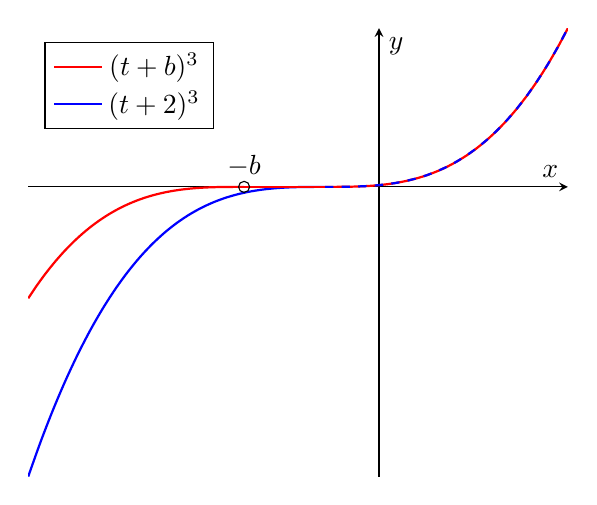
\begin{tikzpicture}
      \begin{axis}[
        domain=-13:7,
        axis x line = center,
        ticks = none,
        % ytick = none,
        axis y line = center,
        xlabel={$x$},
        ylabel={$y$},
        legend pos=north west,
        ]
        \addplot[smooth,color=red,thick,domain=-2:7] {(x + 2)^3};
        \addlegendentry{$(t+b)^3$}
        \addplot[smooth,color=blue,thick,domain=-13:-2] {(x + 2)^3};
        \addlegendentry{$(t + 2)^3$}
        \addplot[smooth,color=red,thick,domain=-5:-2] {0};
        \addplot[smooth,color=red,thick,domain=-13:-5] {(x + 5)^3};
        \addplot[dashed,color=blue,thick,domain=-2:7] {(x + 2)^3};
        \draw (-5,0) circle[radius=2pt] node[above]{$-b$};
      \end{axis}
    \end{tikzpicture}
  \end{center}
  Diese Lösungen sind allesamt linear unabhängig, was zeigt, dass der Satz von Picard-Lindelöf hier eindeutig nicht greift.
\end{Beispiel}

Another one please?


\section{Partielle Differentialgleichungen}

Nun betrachten wir (das deutlich komplexere) Problem: \textbf{Die quasilineare PDE in 2 Variablen}. (partial differential equation)

Wir suchen nun eine unbekannte Funktion $u = u(x,y)$ mit
$$F(x,y,u,u_x,u_y) = 0$$
Also ist $F$ eine Funktion in 5 Variablen, und muss linear in den beiden partiellen Ableitungen sein. Wir könnten auch schreiben
$$a(x,y,u) \cdot u_x + b(x,y,u) \cdot u_y = c(x,y,u) \Leftrightarrow a(x,y,u) \cdot u_x + b(x,y,u) \cdot u_y - c(x,y,u) = 0$$
Schreiben wir nun:
$$F(x,y,z) = \begin{pmatrix}
  a(x,y,z) \\ b(x,y,z) \\ c(x,y,z)
\end{pmatrix}$$
Nun ist
$$n(x,y,z) = \begin{pmatrix}
  ux \\ u_y \\ -1
\end{pmatrix}$$
ein Normalenvektor an den Graphen von $u$ im Punkt $(x,y,z)$. Wir können auch sagen
$$n(x,y,z) = grad(u(x,y) - z)$$
Unser Differentialgleichung wird zu
$$<F(x,y,u),n(x,y,u)> = 0$$
Der Graph von $u$ fließt entlang dem Vekorfeld $F$, also:

Für alle $(x,y,z)$ im Graphen von $u$ (Fläche in $\R³$) ist $F(x,y,z)$ Tangential an den Graphen.


\begin{Theorem}[Cauchy-Kovalerskaya]
  Sei $F = \left(\begin{smallmatrix}
    a \\ b \\ c
  \end{smallmatrix}\right)$ ein Vektorfeld auf (einer offenen Menge in) $\R³$ mit $a(x,y,z) \neq 0$. Dann hat die Differentialgleichung
  $$\left\{\begin{aligned}
    a \cdot u_x + b \cdot u_y & = c \\
    u(0,y) & = f(y)
  \end{aligned}\right.$$
  ($f$ von Klasse $\mathcal{C}¹$)

  eine \textbf{eindeutige} Lösung für kleine $x$. (also $|x| < T(y)$).
\end{Theorem}

\subsection{Allgemeine partielle Differentialgleichungen}

Königsklasse der DGLs, wir besitzen noch nicht die nötigen Werkzeuge, um mit ihnen umzugehen. Sie bieten meistens genug Stoff für eine Dokorarbeit, als einzelne Gleichung.

Wir betrachten lediglich ein Beispiel 'aus dem Alltag' und kratzen so erst an der Oberfläche eines riesigen Teilgebiets der Mathematik.

\begin{Beispiel}[Isoperimetrische Probleme]
  Folgende einfache Frage: Welche ist die flach berandete Fläche mit dem größten Volumen bei fixem Umfang?

  Betrachten wir das Problem nur im 2-dimensionalen, so ist die Antwort: Der Kreis. Aber wieso?

  Behandelt wurden Beweise:
  \begin{enumerate}
    \item ...von Steiner, als geometrische Intuition. Der Beweis stellt sich allerdings als logisch falsch verankert heraus.
    \item ...über ??? Es treten die Euler-Lagrange Sätze auf, die sich unter diesen speziellen Bedingungen 'relativ' einfach lösen lassen.
    \item ...über Fourier-Analyse. Betrachten wir den Vektorraum der periodischen Funktionen in $\C$ (also, die auf $[0,1\pi]$ eine Schleife bilden), so können wir den Umfang im Verhältnis zur Fläche minimieren. Auch das entspricht einer Differentialgleichung, die sich dank der Fourier-Koeffizienten drastisch kürzt.
  \end{enumerate}

  Diese Beweise lassen sich wohl schwer erweitern und deshalb betrachten wir noch den Ansatz über geometrische Integration, der sich letzten Endes auf das Nadelproblem von Bouffon zurückführen lässt (wie hoch ist die Wahrscheinlichkeit, dass eine geworfene Nadel über der Naht eines aus Rechtecken bestehenden Bodens liegen bleibt?). Aus sicherer Quelle gilt, dass man mit diesen Überlegegungen auch in verschiedenen Räumen auf Lösungen kommt.
\end{Beispiel}

\end{document}
